\section{Introduzione}
    Fino ad ora abbiamo considerato i processi come aventi un unico processo di controllo. Tuttavia questo non è vero nella maggior parte dei sistemi operativi moderi, in quanto essi dispongono di più processi di controllo all'interno dello stesso processo chiamati \textbf{thread}. Con l'aumentare dei core è importante identificare opportunità di parallelismo per aumentare, talvolta drasticamente, le performance del sistema.
    
    Un \textbf{thread} è l'unità di base d'uso della CPU e comprende un identificatore di thread (ID), un contatore di programma, un insieme di registri e una pila (\textit{stack}). Condivide con gli altri thread che appartengono allo stesso processo al sezione del codice, la sezione dei dati e altre risorse di sistema come file aperti e segnali. Un processo tradizionale, chiamato anche \textbf{processo pesante} (\textit{heavyweight process}), è composto da un solo thread. Un processo multithread è capace di svolgere più compiti in maniera concorrente.
    
    \begin{figure}[h]
        \centering
        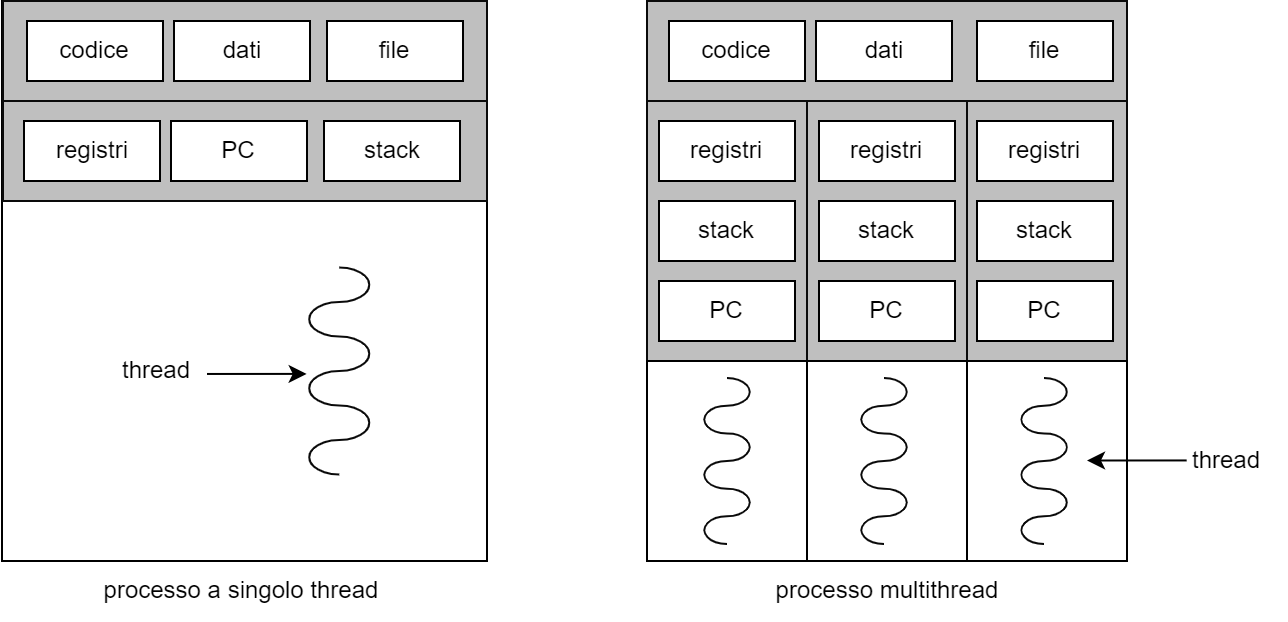
\includegraphics[width=1\textwidth]{img/threads.png}
        \caption{Differenza fra processo a singolo thread e multithread}
        \label{fig:my_label}
    \end{figure}
    
    \subsection{Motivazioni}
        La maggior parte delle applicazioni per computer moderni è \textbf{multithread}. Di solito si codifica come un processo a sé stante comprendente più thread di controllo. Per esempio possiamo avere un'applicazione galleria che usa diversi thread per creare diverse thumbnail, o un browser web che usa thread per rappresentare immagini e testo e uno per scaricare dati dalla rete.
        
        Possiamo pensare, prendendo per esempio un server web utilizzato da moltissimi utenti contemporaneamente, la creazione di un processo che a ogni richiesta utente crea un altro processo che soddisfa la richiesta, per esempio la restituzione di una pagina web. Questa tecnica è stata effettivamente usata per molto tempo, ma questo è un caso in cui molti processi devono eseguire compiti simili fra loro. Creare un processo è dispendioso, e quanto più i compiti che devono eseguire sono simili, tanto meno vale la pena di creare nuovi processi per ogni compito. L'evoluzione naturale di ciò è creare un processo multithread che crea appunto \textbf{thread} per le varie richieste che riceve.
        
        La maggior parte dei kernel è multithread. Durante l'avvio di Linux per esempio sono creati diversi thread e ognuno si occupa di una diversa fase dell'inizializzazione del sistema. Possiamo notare che in Linux abbiamo il thread \texttt{kthreadd} (pid = 2) che funge da genitore di tutti gli altri thread a livello kernel.
        
        Molti algoritmi, come quelli di ordinamento e gli algoritmi per alberi e grafi, possono trovare grandi vantaggi dal multithreading. Ovviamente queste non sono le uniche applicazioni, e anche in ambito di data mining, intelligenza artificiale, grafica etc. possono essere e sono usate tecniche per avvalersi della potenza dei moderni sistemi multicore.
        
    \subsection{Vantaggi}
        I vantaggi della programmazione multithread si possono classificare in quattro categoria principali.
        \begin{enumerate}
            \item \textbf{Tempo di risposta.} Rendere multithread un'applicazione interattiva potrebbe, in casi moderni, essere l'unico modo di garantire una buona esperienza utente, in quanto il sistema può elaborare l'input utente e continuare la sua esecuzione. Si consideri un'interfaccia utente, e in particolare l'utilizzo di un mouse. In un'applicazione a thread singolo il sistema potrebbe gestire il cursore o eseguire funzioni, mentre in un sistema multithread queste cose si possono separare.
            
            \item \textbf{Condivisione delle risorse.} Un processo deve specificare se vuole condividere risorse tramite l'utilizzo di memoria condivisa o scambio di messaggi, mentre i thread dispongono di memoria condivisa di default. Dunque un'applicazione può avere thread che eseguono attività diverse ma hanno accesso allo stesso codice e dati, e tutti nello stesso spazio di indirizzi.
            
            \item \textbf{Economia.} Assegnare memoria e risorse per un nuovo processo può essere costoso, tanto che conviene spesso creare nuovi thread e gestirne il context switch, in quanto essi condividono le stesse risorse e rendono non necessaria una nuova inizializzazione.
            
            \item \textbf{Scalabilità.} Il multithreading su una macchina multicore incrementa il parallelismo. Nel caso di un programma a thread singolo, potremmo sfruttare comunque un solo core per volta, lasciando buona parte delle capacità di computazione del sistema non usate.
        \end{enumerate}
        
\section{Programmazione multicore}
    Nel corso della storia, in risposta a una richiesta di maggiore capacità di calcolo si è passati da sistemi con una singola CPU a sistemi con più CPU, e in seguito a sistemi con più \textit{core} per singolo chip, i quali vengono visti dal sistema operativo come processori separati. Un tipo di programmazione multithread sfrutta molto meglio questo tipo di architettura.
    
    Si noti la differenza fra \textbf{parallelismo} e \textbf{concorrenza}. Un sistema concorrente supporta più task permettendo a ciascuno di progredire nell'esecuzione. Un sistema parallelo invece può eseguire contemporaneamente più task.
    
    \subsection{Tipi di parallelismo}
        In generale, esistono due tipi di parallelismo: parallelismo dei dati e parallelismo delle attività.
        
        Il \textbf{parallelismo dei dati} prevede la suddivisione di una certa mole di dati su più core e l'esecuzione delle stesse operazioni su ogni sottoinsieme dei dati.
        
        Il \textbf{parallelismo delle attività} prevede la distribuzione di attività (thread) su più core, e non di dati. Ogni thread realizza un'operazione distinta, e più thread possono operare sugli stessi dati o su dati diversi.
        
        Questi due tipi di parallelismo non sono mutualmente esclusivi, e le applicazioni possono utilizzare un ibrido di queste due strategie.
        
    \section{Modelli di supporto al multithreading}
        I thread possono essere distinti in \textbf{thread a livello utente} e \textbf{thread a livello kernel}: i primi sono gestiti sopra al livello kernel e senza il suo supporto; i secondi sono gestiti direttamente dal sistema operativo.
        
        In ogni caso deve esistere una relazione fra questi due livelli. Ne analizziamo tre opzioni.
        \begin{figure}[h]
                \centering
                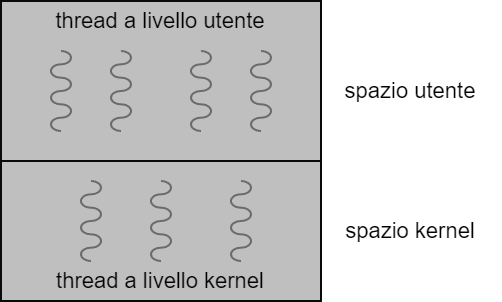
\includegraphics[width=0.5\textwidth]{img/thread1.png}
                \caption{Thread a livello utente e a livello kernel}
                \label{fig:thread1}
            \end{figure}
        
        \subsection{Modello da molti a uno}
            In questo modello, molti thread a livello utente corrispondono a un solo thread a livello kernel. La gestione dei thread risulta efficiente, ma tutto il processo rimane bloccato nel caso in cui un thread invochi una chiamata di sistema di tipo bloccante. Inoltre, poiché un solo thread alla volta può accedere al kernel, è impossibile eseguire thread multipli in sistemi multicore: ne deriva che questo modello è poco utilizzato nei sistemi moderni.
            
            \begin{figure}[h]
                \centering
                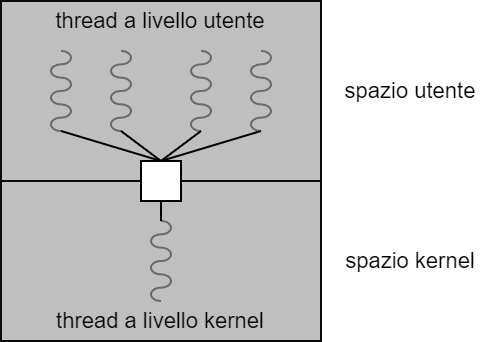
\includegraphics[width=0.5\textwidth]{img/thread2.png}
                \caption{Modello da molti a uno}
                \label{fig:my_label}
            \end{figure}
            
            
        \subsection{Modello da uno a uno}
            Questo modello mette in corrispondenza ciascun thread a livello utente con un thread a livello kernel. Questo modello offre un maggior grado di concorrenza, in quanto anche se un thread effettua una chiamata bloccante è comunque possibile eseguire un altro thread, e inoltre consente anche l'esecuzione parallela di thread in sistemi multiprocessore. Lo svantaggio di questo modello è che per ogni thread a livello utente va creato un thread a livello kernel, e ciò può creare problemi di prestazioni. Infatti nonostante questo modello sia utilizzato su sistemi della famiglia Windows e Linux, c'è un limite al numero di thread che è possibile creare.
            
            \begin{figure}[h]
                \centering
                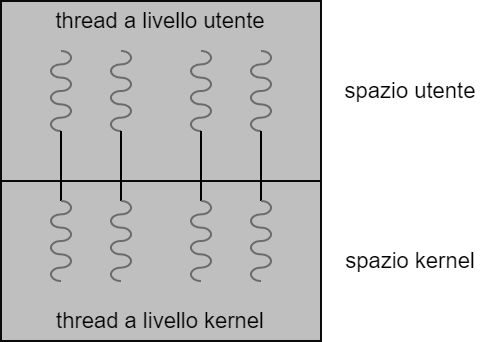
\includegraphics[width=0.5\textwidth]{img/thread3.png}
                \caption{Modello da uno a uno}
                \label{fig:my_label}
            \end{figure}
            
        \subsection{Modello da molti a molti}
            Questo modello mette in corrispondenza un certo numero di thread a livello utente con un numero minore o uguale di thread a livello kernel. Questo numero può variare in base all'applicazione o al calcolatore. Possiamo per esempio assegnare più thread in un'architettura dotata di otto core rispetto a quanti ne verrebbero assegnati in un'architettura dotata di quattro core.
            
            Per quanto riguarda la concorrenza, abbiamo visto che il modello molti a uno non la supporta in quanto possiamo scegliere un solo thread utente alla volta, mentre quello uno a uno la supporta, ma con la clausola di non creare troppi thread. Il modello molti a molti non ha nessuno di questi problemi, in quanto il programmatore può creare tutti i thread che ritiene necessario ed essi possono essere assegnati a diversi thread a livello kernel per l'esecuzione in parallelo. Inoltre una chiamata di sistema bloccante non è un grande problema, in quanto in questo caso il kernel può schedulare un altro thread.
            
            Una variante di questo modello prevede comunque la corrispondenza fra un certo numero di thread utente e un numero minore o uguale di thread kernel, ma permette anche di vincolare un singolo thread utente a un thread kernel. Questa variante è chiamata \textbf{modello a due livelli}.
            
            Nonostante il modello molti a molti sembri il più flessibile, è difficile metterlo in pratica. Inoltre, il limite di thread a livello kernel si alza con l'aumentare dei core di elaborazione, e diventa sempre meno importante.
            
            \begin{figure}[h]
                \centering
                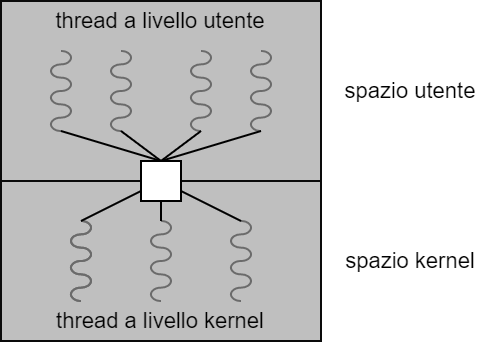
\includegraphics[width=0.7\textwidth]{img/thread4.png}
                \caption{Modello da molti a molti}
                \label{fig:my_label}
            \end{figure}
            
            \newpage
            \begin{figure}
                \centering
                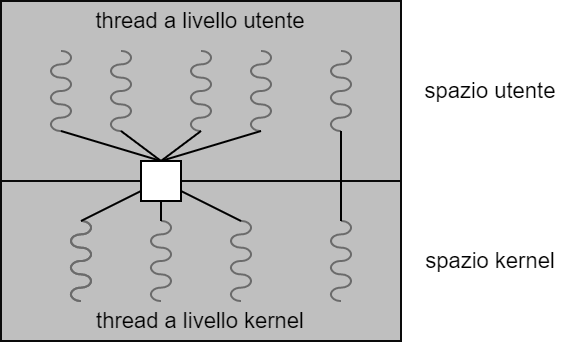
\includegraphics[width=0.7\textwidth]{img/thread5.png}
                \caption{Modello a due livelli}
                \label{fig:my_label}
                \vspace{5.6in}
            \end{figure}